\chapter{Process og projektgennemførsel}

I dette afsnit beskrives gennemførslen af projektet, herunder: process, ledelse samt anvendte principper og værktøjer. Disse principper og værktøjer har været et vigtigt element i udarbejdelsen af systemet, og har haft til formål at give arbejdet struktur samt at hjælpe gruppens til at få et overblik over færdigt og ufærdigt arbejde.

\section{SCRUM og agile udvikling}
Scrum er et ''Agile development'' værktøj \cite[kap. 1]{robertmartin2006}. I dette projekt bruges de grundprincipper, som har været mest logiske for gruppen. Som udgangspunkt er der afholdt et ugentligt møde, hvor gruppen har talt og diskuteret den forrige uges arbejde, samt hvilke problemer eller forhindringer der har været eller kommer.

Gruppen har ikke brugt scrum ''fully dressed'' men har derimod taget de principper og grundsten som gav mening for et mindre team.

\subsection{Milestones}
En af principperne i scrum er at lave det der giver størst værdi. Arbejdet er tilrettelagt efter at lave de vigtigste ting først. Disse blev identificeret ved en \gls{moscow} analyse, se afsnit~\ref{sec:moscow}.

Når et punkt i \gls{moscow} var valgt har hele gruppen så designet og implementeret områder inden for respektive specialisering. På denne måde er der arbejdet iterativt med projektet.

\subsection{Retrospekt}
Løbende har gruppen revideret samarbejdet i forbindelse med gruppemøder. Dette har givet en stærkere team, og forbedret kommunikationen i gruppen.

Eksempelvis kom det i starten frem at gruppemedlemmer havde en tendens til at arbejde på en del af systemet, uden at resten af gruppen var klar over hvad de så tilsvarende skulle lave.
Dette blev heldigvis tidligt bragt op på et møde, så problemet var kendt. Dette ledte til at medlemmerne gjorde meget ud af at tale sammen og koordinere arbejdet på tværs af undergrupperne.

\subsection{Development spikes}
Et princip der også tager udgangspunkt i den agile tankegang. Et development spike \cite{scaledagile} går ud på at der designes og implementeres de nødvendige dele for at et ''signal'' kan gå fra ende til anden i systemet.

Dette princip har været brugt i starten, før \gls{db}, \gls{windserver} og diverse klienter kunne tale sammen om en opgave. På denne måde kom et grundlæggende system på benene. På dette tidspunkt handlede det \textit{kun} at der skulle tilføjes mere funktionalitet.

\section{User Stories}
På tidligere semestre har use cases været brugt til at vise scenarier for hvordan systemet kan bruges. I dette projekt bruges user stories \cite{margaretrouse2015}, som er en kort beskrivelse af en system-feature. En \gls{us} skal forstås som et ønske fra slutbrugerens side, og er altså derved en beskrivelse af et systemkrav.

\subsection{Pivotal Tracker}
Pivotal Tracker er et webbaseret, agilt projektsstyrings værktøj, udviklet af pivotal labs. Pivotal tracker stiller et interaktivt scrumboard til rådighed, hvorpå der er mulighed for at tilføje user-stories til en backlog, tracke teamets velocity samt se opgaver der er færdige. Figur~\ref{fig:scrumboard} viser et eksempel på gruppens Pivotal Tracker side.

\begin{figure}
	\centering
	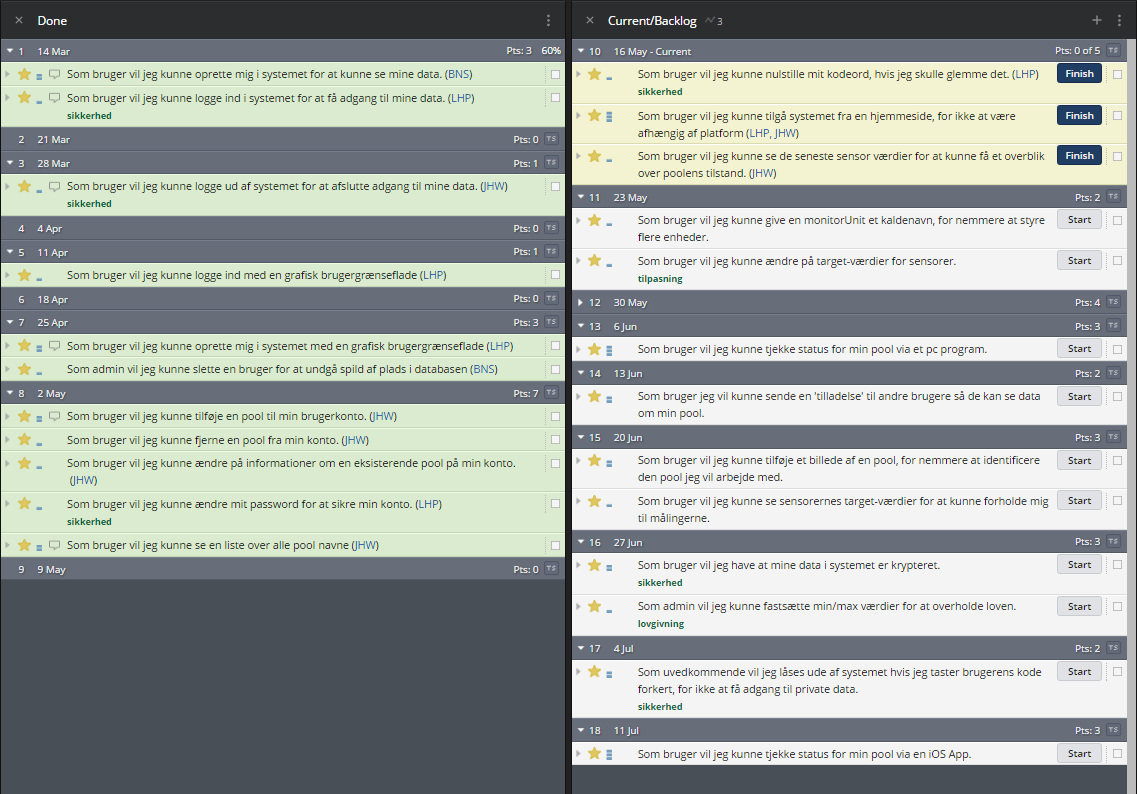
\includegraphics[width=\linewidth]{figs/processProjektGennemforsel/scrumboard.PNG}
	\caption{Pivotal tracker's interaktive scrumboard}
	\label{fig:scrumboard}
\end{figure}

 Da user-stories er meget generelle i forhold til use cases, er der mulighed for at tilføje specificerede tasks til hver user story og på den måde bryde en user-story ned i mindre dele så hele opgaven bliver mere overskuelig.

\begin{figure}
	\centering
	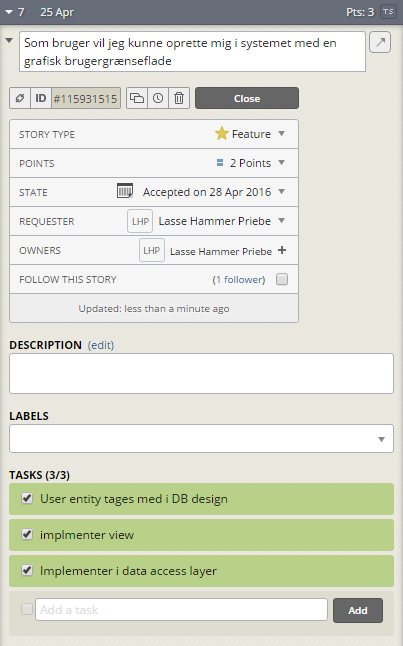
\includegraphics[width=0.6\linewidth]{figs/processProjektGennemforsel/userstory_with_tasks.PNG}
	\caption{User Story - Opret Bruger}
	\label{fig:userstory_with_tasks}
\end{figure}

Som det ses på figur~\ref{fig:userstory_with_tasks} giver Pivotal Tracker mulighed for at tjekke tasks af efterhånden som de udføres. Når der tages hul på en opgave i Pivotal Tracker trykkes der på knappen Start, hvorefter den pågældende user story markeres som påbegyndt. Når alle tasks i den pågældende userstory er færdige kan udvikleren trykke på knappen Deliver. Herefter kan der startes på en ny opgave.

\subsubsection{Estimering}
Når der i fællesskab udarbejdes user stories, bliver teamet samtidig enige om en tidsestimering. I Pivotal Tracker er der mulighed for at give en \gls{us} henholdsvis 1, 2 og 3 point alt efter hvor lang tid, det anslås at der skal bruges på at udvikle denne feature.
Som det kan ses på figur~\ref{fig:userstory_with_tasks} er der tildelt 2 point til en \gls{us}. Dette er grundet behovet for udvikling af både database, Data Access Layer, samt GUI. Altså er det en feature der berører alle aspekter af projektet.

\section{Test Driven Development}
TDD er en udviklingsmetode, som foreskriver at test skrives før selve produktionskoden \cite{osherove2015art}. Gruppen har ikke brugt TDD 100\% gennemforløbet. 
Dog har TDD været særligt brugbart i udviklingen af DAL\footnote{Data Access Layer} laget, idet at de enkelte methoder har været enkle nok til der kunne skrives test før selve produktionskoden skulle skrives.

\section{Versionsstyring}
En fuldstændig essentiel del af softwareudvikling er versionstyring. Det er et værktøj der giver mulighed for at flere udviklere kan arbejde, tæt sammen, på et projekt uden at træde hinanden over tæerne.\todo{bedre formulering?}

\subsection{Git}
Gruppen har igennem hele forløbet benyttet versionsstyrings-værktøjet Git. Git er gratis, og har været brugt i kurser som Software Test og Indlejret Software Udvikling. 

Git bruges i projektet til al source kode, og hver feature udvikles på sin egen branch for at undgå konflikter. Når en feature er færdig udstedes et pull request, hvorefter repository administratoren kan merge koden ind på master branch.

For at holde styr på branches og versioner er der brugt Feature Branching \cite{atlassian2016}. Dette indebære der ikke foregår noget produktionsarbejde på master branchen. I stedet skal der oprettes en branch specielt til denne feature. Så når denne feature er testet med seneste udgave af master branchen, kan ændringerne blive ''merget'' ind. På denne måde har gruppen hele tiden haft en fungerende produkt at vise frem, hvis det skulle blive nødvendigt.

\subsubsection{GitHub}
Github er online hosting af Git repositories, og er brugt i projektet til at gemme source kode, samt administrere projektets repository. I forbindelse med projektstyring og adminitration, har git været brugt til eksempelvis at tracke teamets effektivitet og commit-frekvens.

\subsection{Travis CI og Jenkins}
Gruppen har undervejs forsøgts sig med både med Travis CI og Jenkins. Da gruppen allerede var godt bekendt med Jenkins, virkede Travis CI som en interessant mulighed for at prøve noget anderledes.
Begge værktøjer er til continuos integration. CI er belejligt idet en ekstern server står for at bygge al source kode der bliver pushet til projektets repository og kører tilsvarende tests.

Dette er især nyttigt til større projekter, hvor lokale test på udviklerens computer ikke er hensigtsmæssige af tidsmæssige årsager. Travis CI er gratis til offentlige repositories på GitHub. Dog er Travis CI kun ''community supported'' for C\# kode \cite{communitysupportedlanguages2016}, hvilket præsenterede en udfordring.

Da projektet både indeholder en applikation til PC, iOS og en web applikation, har det været en udfordring at benytte et continous integration værktøj.
Dette kombineret med at hele testsuiten hurtigt kunne eksekveres lokalt, ledte til at gruppen valgte at prioritere tid brugt på udvikling og lokale test.

Dette har dog ikke forhindret et forsøg. Det lykkedes gruppen at sætte den ellers kun ''community supported'' Travis CI op til at teste et C\# projekt fra github, som skulle konstatere om der skulle bruges mere tid på Travis CI. 

Til et github projekt skal der tilføjes en \textit{.travis.yml}-fil. Denne bestemmer hvilke pakker mm. der skal installeres og hvilke test der skal køres. 
Herefter lykkedes det at sætte github repositoriet op til kun at tillade et merge hvis koden kan bygge og består alle tests som vist på figur~\ref{fig:travispullrequest}.

\begin{figure}[h]
	\centering
	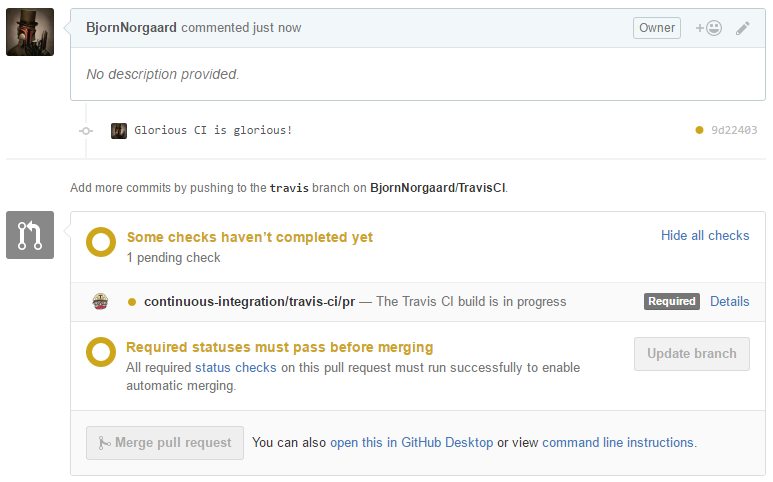
\includegraphics[width=0.9\linewidth]{figs/processProjektGennemforsel/travis/travispullrequest}
	\caption{Github's menu når der laves et pull request.}
	\label{fig:travispullrequest}
\end{figure}

Når Travis CI så har bygget og testet kan koden blive merget ind i master, se figur~\ref{fig:travisgithubsuccess}.

\begin{figure}[h]
	\centering
	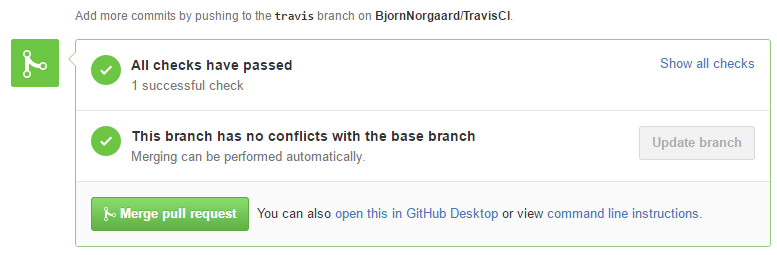
\includegraphics[width=0.9\linewidth]{figs/processProjektGennemforsel/travis/travisgithubsuccess}
	\caption{Github pull request, efter at alle test er kørt med Travis CI.}
	\label{fig:travisgithubsuccess}
\end{figure}

\section{Software test}
Software testing har været en stor del af dette projekt. Der har været stor fokus på robusthed. Der er i alt skrevet cirka 200 automatiserede tests, se figur~\ref{fig:vsUnittest}. Af disse er lidt over halvdelen skrevet til DAL, som er den mest oplagte del at enhedsteste, da eksempelvis GUI laget hovedsageligt er testet visuelt.

\begin{figure}[h]
	\centering
	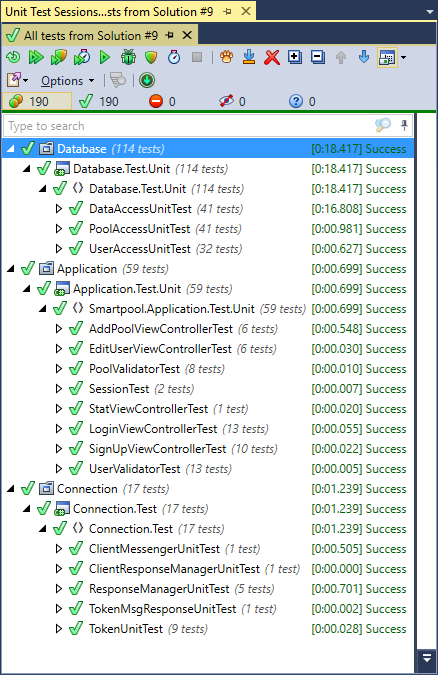
\includegraphics[width=0.5\linewidth]{figs/processProjektGennemforsel/vsUnittest}
	\caption{Unitest session i Visual Studio}
	\label{fig:vsUnittest}
\end{figure}

\subsection{NUnit- og testframeworks}\todo{Afsnittet skal muligvis flyttes til Udviklingsværktøjer...}
Et oplagt værktøj til softwaretest har været Nunit idet det bruges i vid udstrækning i forbindelse med kurset Software Test.

\section{UML}
UML er brugt i vid udstrækning gennem alle projektets faser. UML danner grundstenen i projektets dokumentation, men har også hjulpet udviklingen undervejs, idet visualiseringen har givet en bedre forståelse og gør det lettere at gennemskue nye og smartere designmuligheder.

\section{Gruppeledelse og -struktur}
Ledelsesstrukturen har hovedsageligt været flad. Gruppemedlemmer har i fællesskab afgjort hvilke elementer af projekt der har været vigtigst, og derefter selv fundet de bedste måder at implementere disse på.

I forbindelse med gruppemøder har der imidlertid ofte været én som agerede ordstyre. Dette var for at begrænse tiden mødet skulle tage, sådan at både vejleder og medlemmer hurtigt kunne kommer videre til andre opgaver.